\documentclass{beamer}
\usetheme{Ilmenau}
\usecolortheme{default}
\usefonttheme{serif}

\usepackage{lipsum}
\usepackage{graphicx,xcolor,tikz}
\usepackage{amsmath,amssymb,amsfonts}
\usetikzlibrary{automata} % LATEX and plain TEX
\usetikzlibrary[automata] % ConTEXt
\usepackage{comment}
\usepackage{rotating}
\usepackage[export]{adjustbox}

\newtheorem{thm}{Theorem}
\newtheorem{dfn}{Definition}

\newcommand{\ds}{\displaystyle}
\newcommand{\R}{{\mathbb R}}
\newcommand{\Q}{{\mathbb Q}}
\newcommand{\Z}{{\mathbb Z}}
\newcommand{\N}{{\mathbb N}}
\newcommand{\C}{{\mathbb C}}
\DeclareMathOperator{\Ap}{Ap}
\DeclareMathOperator{\PF}{PF}
\DeclareMathOperator{\KC}{KC}

\usepackage[mathscr]{euscript}
\usepackage{stackrel}
\usepackage{comment}

\setbeamertemplate{footline}[frame number]{}
\setbeamertemplate{navigation symbols}{}

\defbeamertemplate*{headline}{split theme}
{}


\title{Pflueger's Conjecture for Numerical Semigroups of Small Depths\\[5pt]\footnotesize{\textit{Cal-Bridge UCI Fall Conference}}}
\author[Wiest]{Victoria Wiest\\ Advised by Dr. Nathan Kaplan}
\institute[Fresno State]{California State University, Fresno}
\date{}

\begin{document}

\begin{frame}
\titlepage
\end{frame}

\section{Preliminaries}
\begin{frame}{Numerical Semigroups}
    A nonempty subset of $\N_{0}=\{0,1,2,3,\dots\}$, denoted as $S$, is a \textbf{numerical semigroup}, if and only if

    \begin{itemize}
        \item $0\in S$,
        \item $\N_{0} - S$ is finite, and
        \item If $x\in S$ and $y\in S$, then $x+y\in S$ (closed under addition)
    \end{itemize}\vspace{8pt}
    Ex: $\{0,3,4,6,7,8,\to\}$
    
\end{frame}

\begin{frame}{Apery Set}

\[S=\{0,4,6,8,9,10,12,13,14,15,\to\}\]

    \begin{center}
    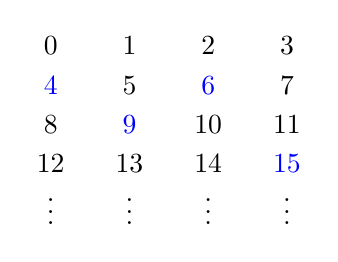
\begin{tikzpicture}
        \node at (0.5, 2) {$0$}; 
        \node at (1.5, 2) {$1$}; 
        \node at (2.5, 2) {$2$}; 
        \node at (3.5, 2) {$3$}; 
        \node at (0.5, 1.5) {\textcolor{blue}{$4$}}; 
        \node at (1.5, 1.5) {$5$}; 
        \node at (2.5, 1.5) {\textcolor{blue}{$6$}}; 
        \node at (3.5, 1.5) {$7$}; 
        \node at (0.5, 1) {$8$}; 
        \node at (1.5, 1) {\textcolor{blue}{$9$}}; 
        \node at (2.5, 1) {$10$}; 
        \node at (3.5, 1) {$11$}; 
        \node at (0.5, 0.5) {$12$}; 
        \node at (1.5, 0.5) {$13$}; 
        \node at (2.5, 0.5) {$14$}; 
        \node at (3.5, 0.5) {\textcolor{blue}{$15$}}; 
        \node at (0.5, 0) {\vdots}; 
        \node at (1.5, 0) {\vdots}; 
        \node at (2.5, 0) {\vdots}; 
        \node at (3.5, 0) {\vdots};
    \end{tikzpicture}
    \end{center}
\end{frame}

\begin{frame}{Apery Set}

\[S=\{0,4,6,8,9,10,12,13,14,15,\to\}\]

    \begin{center}
    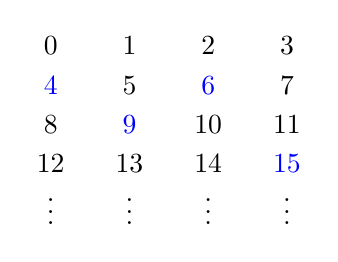
\begin{tikzpicture}
        \node at (0.5, 2) {$0$}; 
        \node at (1.5, 2) {$1$}; 
        \node at (2.5, 2) {$2$}; 
        \node at (3.5, 2) {$3$}; 
        \node at (0.5, 1.5) {\textcolor{blue}{$4$}}; 
        \node at (1.5, 1.5) {$5$}; 
        \node at (2.5, 1.5) {\textcolor{blue}{$6$}}; 
        \node at (3.5, 1.5) {$7$}; 
        \node at (0.5, 1) {$8$}; 
        \node at (1.5, 1) {\textcolor{blue}{$9$}}; 
        \node at (2.5, 1) {$10$}; 
        \node at (3.5, 1) {$11$}; 
        \node at (0.5, 0.5) {$12$}; 
        \node at (1.5, 0.5) {$13$}; 
        \node at (2.5, 0.5) {$14$}; 
        \node at (3.5, 0.5) {\textcolor{blue}{$15$}}; 
        \node at (0.5, 0) {\vdots}; 
        \node at (1.5, 0) {\vdots}; 
        \node at (2.5, 0) {\vdots}; 
        \node at (3.5, 0) {\vdots};
    \end{tikzpicture}
    \end{center}\vspace{8pt}
    Apery set of $S$ is 
    \begin{align*}
        \Ap(S,4)&=\{0,9,6,15\}\\
                &=\{0,2\cdot 4+1,1\cdot 4+2,3\cdot 4+3\}
    \end{align*}
\end{frame}

\begin{frame}{Apery tuple/Kunz coordinate vector}

\[S=\{0,4,6,8,9,10,12,13,14,15,\to\}\]
\begin{center}
    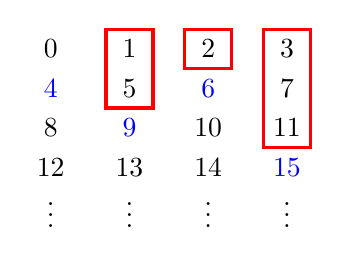
\begin{tikzpicture}
        \node at (0.5, 2) {$0$}; 
        \node at (1.5, 2) {$1$}; 
        \node at (2.5, 2) {$2$}; 
        \node at (3.5, 2) {$3$}; 
        \node at (0.5, 1.5) {\textcolor{blue}{$4$}}; 
        \node at (1.5, 1.5) {$5$}; 
        \node at (2.5, 1.5) {\textcolor{blue}{$6$}}; 
        \node at (3.5, 1.5) {$7$}; 
        \node at (0.5, 1) {$8$}; 
        \node at (1.5, 1) {\textcolor{blue}{$9$}}; 
        \node at (2.5, 1) {$10$}; 
        \node at (3.5, 1) {$11$}; 
        \node at (0.5, 0.5) {$12$}; 
        \node at (1.5, 0.5) {$13$}; 
        \node at (2.5, 0.5) {$14$}; 
        \node at (3.5, 0.5) {\textcolor{blue}{$15$}}; 
        \node at (0.5, 0) {\vdots}; 
        \node at (1.5, 0) {\vdots}; 
        \node at (2.5, 0) {\vdots}; 
        \node at (3.5, 0) {\vdots};

    \draw[red, very thick] (1.2,1.25) rectangle (1.8,2.25);
    \draw[red, very thick] (2.2,1.75) rectangle (2.8,2.25);
    \draw[red, very thick] (3.2,0.75) rectangle (3.8,2.25);

    \end{tikzpicture}
\end{center}

    The Apery set of $S$ is 
    \begin{align*}
        \Ap(S,4)&=\{0,9,6,15\}\\
                &=\{0,\textcolor{red}{2}\cdot 4+1,\textcolor{red}{1}\cdot 4+2,\textcolor{red}{3}\cdot 4+3\}
    \end{align*}

    The Apery tuple or Kunz coordinate vector of $S$ is 
    \[\KC(S,4)=(\textcolor{red}{2},\textcolor{red}{1},\textcolor{red}{3})\]
    
\end{frame}

\section{Acknowledgments}
\begin{frame}{Acknowledgments}
I would like to give a big thank you to:
\begin{itemize}
    \item 
\end{itemize}
\begin{columns}[c]
            \begin{column}{.25\textwidth}
            \begin{figure}
                \centering
                \includegraphics[width=0.6\textwidth]{Victoria/Kunz Presentation/CSU,Fresno.png}
            \end{figure}      
            \end{column}
            \begin{column}{.25\textwidth}
            \begin{figure}
                \centering
                \includegraphics[width=1.2\textwidth]{Victoria/Kunz Presentation/Cal-Bridge.jpg}
            \end{figure}
            \end{column}
        \end{columns}

\end{frame}

\end{document}
